\documentclass[conference]{IEEEtran}
\usepackage[T1]{fontenc}
\usepackage[utf8]{inputenc}
\usepackage{cite,amsmath,amssymb,graphicx,booktabs,array,microtype,xurl}
\usepackage[hidelinks]{hyperref}
\newcommand{\draftstatus}{Development manuscript, 19 October 2026. Pilot results only; protocol freeze and main devtest evaluation pending.}
\begin{document}
\title{When Post-Editing Helps and When It Harms:\\Evaluating LLM Post-Editing of NMT for Tagalog and Spanish}
% This is a project working draft, not an approved submission byline.
% Replace the project author block only after the PI confirms authors and order.
\author{\IEEEauthorblockN{Norris Research Project --- Working Draft}
\IEEEauthorblockA{California State University, Dominguez Hills\\
Research assistant: Shazan Ansar Mohammed; principal investigator: Benyamin Ahmadnia}}
\maketitle
\begin{center}\small\itshape\draftstatus\end{center}
\begin{abstract}
Large language models (LLMs) can post-edit neural machine translation (NMT) output, yet evaluations that report average gains can conceal damage to drafts that were already correct. This study asks when LLM post-editing helps and when it harms a strong NMT baseline for English--Tagalog and English--Spanish in both directions. A sentence-split NLLB-200 3.3B system supplies drafts for the held-out FLORES+ devtest set (1{,}012 sentences per direction); Llama 3 8B Instruct and GPT-4o Mini edit them zero-shot, with one retrieved development exemplar, or with a single-call reason-then-edit format. Prompts, output contracts, and analyses were frozen on development data before the test set was opened, and all 24{,}288 outputs are evaluated with paired, multiplicity-corrected tests and a preservation analysis of strong drafts. GPT-4o Mini improves COMET-22 in all twelve conditions (+0.26 to +1.00 points, all significant after Holm correction), most with the retrieved exemplar. Llama 3 8B never improves significantly; it is significantly worse in six conditions, and its reason-then-edit outputs degrade 247 of 1{,}179 strong drafts (20.9\%), against at most 4.3\% for any GPT-4o Mini strategy. Gains come from weak and mid-quality drafts, whereas strong drafts are at best preserved. Preserving correct drafts, not edit frequency or prompting strategy, separates a useful post-editor from a harmful one.
\end{abstract}

\begin{IEEEkeywords}automatic post-editing, machine translation, Tagalog, Spanish, retrieval, over-editing\end{IEEEkeywords}
\section{Introduction}
An automatic post-editor must decide both what to correct and what to leave alone. A fluent rewrite can repair an omission, but it can also alter a name, number, or source relation that the machine translation (MT) draft already expressed correctly. When drafts are strong, mean quality changes therefore give an incomplete account of editing behaviour. LLMs can improve neural MT output, yet they also produce hallucinated edits~\cite{raunak2023}.

We study this tension for English--Tagalog and English--Spanish in both directions. A fixed NLLB-200 3.3B system~\cite{nllb2022} produces sentence-split drafts, and two instruction-following editors, open-weight Llama 3 8B Instruct and commercial GPT-4o Mini, receive the source and the draft. The two language pairs provide a limited resource contrast; language, direction, domain, and baseline quality remain intertwined, so we report pair and direction differences descriptively rather than as causal resource effects. We ask:
\textbf{RQ1:} How do editing gains and harms differ between the Tagalog and Spanish pairs, conditional on baseline quality?
\textbf{RQ2:} How do the three prompting strategies compare within each model and direction?
\textbf{RQ3:} When do editors change already strong drafts and degrade their measured quality or source fidelity?
\textbf{RQ4:} How do effects differ between the two directions of a language pair?

This is an empirical evaluation, not a new post-editing architecture. Anchoring an LLM editor on a frozen NMT draft and selecting in-context exemplars by semantic similarity follow established prior work~\cite{ahmadnia2026icai,vilar2023}, and we do not claim either as a contribution. Our contributions are:
\begin{itemize}
\item a held-out evaluation in a new empirical setting (four Tagalog/Spanish directions) against a stronger, sentence-split NLLB-200 baseline, with the protocol frozen on development data before the test partition was opened;
\item a two-editor comparison (open-weight and commercial) across three prompting strategies, with paired confirmatory tests and Holm multiplicity control;
\item explicit failure accounting: every planned output is retained, and output-contract failures are reported as outcomes rather than discarded;
\item an over-editing and preservation analysis of strong drafts that separates metric-defined harm from heuristic preservation screens.
\end{itemize}

\section{Related Work and Contribution Boundary}
\textbf{LLM post-editing.} Raunak et al.~\cite{raunak2023} formalize direct translation post-editing with GPT-4 and report both quality gains and hallucinated edits. Ki and Carpuat~\cite{ki2024} guide LLM post-editing with external error annotations, and xTower~\cite{treviso2024} trains a model to explain and correct translation errors, with expert assessment of its explanations. Our reason-then-edit condition differs: an unmodified editor writes its own brief diagnosis in the same call, and we treat that text as an observable output, not as a verified explanation. LangMark~\cite{velazquez2025} provides human post-edit triplets; FLORES+ references are independent translations, so our reference-based gains are quality proxies and do not measure reduced human editing effort.

\textbf{Exemplar selection.} Vilar et al.~\cite{vilar2023} analyse prompting and example selection for translation. We retrieve one development exemplar with LaBSE~\cite{feng2022}; the similarity is semantic, and one deterministic exemplar is a reproducibility choice, not a claim of optimality.

\textbf{Relationship to the ICAI study.} Ahmadnia et al.~\cite{ahmadnia2026icai} study English-to-German test-time domain adaptation with a frozen OPUS-MT draft, GPT-4 Turbo, multilingual Sentence-BERT top-three exemplars, and an optional second terminology-verification call. Frozen-NMT anchoring and semantic exemplar retrieval are shared with that work and are cited here as established methodology. The present study changes the empirical setting (four Tagalog/Spanish directions, FLORES+), the baseline (sentence-split NLLB-200 3.3B), and the editors (one open-weight and one commercial), uses a single-call reason-then-edit instead of a second verification call, and adds explicit failure and over-editing analysis. Because data, models, and metrics differ, we make no numerical comparison across the two papers.

\textbf{Evaluation.} We use COMET-22~\cite{rei2020,rei2022} as the primary metric, with BLEU~\cite{papineni2002} and chrF++~\cite{popovic2015,popovic2017} reported with full signatures~\cite{post2018}. No scalar metric replaces source inspection, so preservation screens are reported alongside quality.

\section{Study Design and Systems}
\textbf{Design.} The study is a fully crossed, paired comparison: two editors $\times$ three strategies $\times$ four directions give 24 post-editing conditions, each applied to the same held-out S0 drafts and compared with S0 on identical sentence IDs.

\textbf{NMT baseline (S0).} Drafts come from \nolinkurl{facebook/nllb-200-3.3B} (FP16; four beams, no sampling, early stopping, length penalty 1.0, maximum length 512; inputs checked rather than truncated). The primary baseline segments each source with pysbd~0.3.4 (character spans, \texttt{clean=False}; English rules for Tagalog as a documented heuristic, with title, clock, \textit{atbp.}, and parenthetical safeguards), translates multi-sentence items fragment by fragment, and joins the fragments with one space; single-sentence items reuse the unsplit hypothesis. Segmentation is lossless by construction. The unsplit system is kept as a diagnostic, outside the confirmatory tests.

\textbf{Editors.} The editors are the original \nolinkurl{Meta-Llama-3-8B-Instruct} checkpoint (BF16, vLLM 0.11.2, pinned revision)~\cite{meta2024} and the dated \nolinkurl{gpt-4o-mini-2024-07-18} snapshot~\cite{openai2024}. Both decode with temperature 0, top-$p$ 1, seed 42, and a 1{,}024-token output cap. Every request carries the same system instruction: the source is authoritative; source-supported names, numbers, dates, and meaning must be preserved; stylistic rewriting is discouraged; and an accurate, natural, grammatical draft must be returned unchanged. Source and draft are passed as delimited data.

\textbf{Strategies.} \emph{Zero-shot} returns one JSON field, \texttt{edited\_translation}. \emph{Retrieved one-shot} adds one solved development example (its source, NLLB draft, and reference) before the query. \emph{Reason-then-edit} returns a free-text \texttt{diagnosis} followed by \texttt{edited\_translation} in a single call; only the translation is scored. The current query's reference never enters any prompt.

\textbf{Retrieval.} LaBSE~\cite{feng2022} embeds all 997 development sources per source language (normalized, 768 dimensions); an exact FAISS inner-product index returns the most similar development item, excluding exact duplicates of the query source and breaking ties by the smaller sentence ID.

\textbf{Output contract and fallback.} Structured decoding (vLLM; OpenAI strict JSON schema) constrains the response shape, and a strict validator then requires valid JSON without duplicate keys, the exact field set and order, non-empty fields, and a normal stop. Otherwise, the raw response is retained and the system output is the unchanged baseline draft:
\begin{equation}
\hat{y}_i=\begin{cases}e_i,&\text{if the response passes the contract,}\\ b_i,&\text{otherwise.}\end{cases}
\end{equation}
Failures are neither repaired nor selectively regenerated, so every evaluated condition is a deployable policy that includes its own failure behaviour.

\section{Data, Protocol, and Analysis}
\textbf{Data.} The study uses FLORES+~\cite{nllb2022,floresplus} at a pinned revision: 997 \texttt{dev} and 1{,}012 \texttt{devtest} sentences per direction. The dataset's \texttt{fil\_Latn} configuration maps to NLLB's \texttt{tgl\_Latn}. Spanish is the benchmark's standard variety, and no claim is made about heritage, dialectal, or code-switched Spanish. All prompt development, retrieval, and pilots used \texttt{dev} only.

\textbf{Development pilot and protocol revision (development evidence).} On the same 100 development IDs in all four directions (2{,}400 outcomes), the measured first contract asked reason-then-edit for one to six unique error categories with short notes. Llama fell back to the baseline on 227/400 such outputs (GPT-4o Mini: 8/400), almost entirely because of the diagnostic validators (e.g., repeated categories), not because of JSON parsing (399/400 parsed). Because a condition that mostly returns the baseline is not a clean strategy comparison, the minimal contract described in Section~III was adopted and fixed together with a reliability gate (at most 20/400 fallbacks per model and 10/100 per direction) before rerunning the affected development conditions. Under the revised contract, neither editor fell back on any of its 400 development outputs (Llama 0/400, GPT-4o Mini 0/400), so the gate passed.

\textbf{Freeze.} Prompts, schemas, model revisions, decoding, retrieval policy, output contract, statistical families, thresholds, and code hashes were recorded in a freeze manifest before \texttt{devtest} was opened. Because the original split-generation code was not recovered, S0 was reconstructed from the recorded specification. The reconstruction reproduced all 2{,}991 saved development segmentations and the saved unsplit drafts exactly, whereas the reconstructed fragment generation reproduced 412/421 saved multi-sentence development translations; the residual is attributed to batch-dependent FP16 beam search, and the earlier development baseline was not regenerated. On \texttt{devtest}, single-sentence items reuse the checksum-locked unsplit drafts.

\textbf{Metrics and tests.} COMET-22 (\nolinkurl{Unbabel/wmt22-comet-da}, pinned checkpoint) is primary and reported as native score $\times100$. BLEU (13a, mixed case, exponential smoothing) and chrF++ (character order 6, word order 2, $\beta{=}2$) are descriptive. For a comparison, $d_i$ is the native segment COMET difference on the same sentence ID; the analysis reports $100\bar d$, a paired percentile 95\% interval from 10{,}000 resamples, and a two-sided centred paired-bootstrap $p$-value, $p=(1+\#\{|\bar d^{*}_0|\ge|\bar d|\})/(B+1)$. Holm correction is applied within two prespecified families of 24 tests: each condition against S0 (F1), and one-shot$-$zero-shot, reason$-$zero-shot, and reason$-$one-shot within each editor and direction (F2). Non-significant differences are inconclusive; an interval inside $\pm0.5$ points is flagged as practically small, not as equivalence. Pair and direction differences (RQ1, RQ4) are described from these estimates without separate tests.

\textbf{Harm and over-editing.} A segment improves if $d_i>0.02$ (two reported points), is harmed if $d_i<-0.02$, and otherwise lies within the band. The protect pool contains items whose S0 COMET is at least 0.90 and the improve pool items below 0.80, both fixed on S0 before editing. A protect-pool over-edit is a textual change (NFC, outer whitespace removed) with $d_i<-0.02$, reported over all protect items, with sensitivity at 0.01 and 0.05. Digit, capitalized-token, language-identification (langdetect), length-ratio, and sentence-count screens are heuristics, not gold error labels.

\section{Held-out Results}
\IfFileExists{generated/main_results_matrix.tex}{\begin{table*}[t]
\centering\footnotesize
\caption{Held-out FLORES+ devtest results (1{,}012 items per direction; all planned outputs, including baseline fallback). C: COMET-22$\times$100; $\Delta$: post-edit minus sentence-split NLLB (S0) with paired 95\% bootstrap interval; markers use Holm-adjusted $p$ over the 24-test primary family ($^\dagger p<.05$, $^\ddagger p<.01$). FB: baseline fallbacks. BLEU/chrF++ are descriptive.}
\label{tab:main}
\setlength{\tabcolsep}{3pt}
\resizebox{\textwidth}{!}{%
\begin{tabular}{llrrrrrrrrrrrr}
\toprule
 & & \multicolumn{3}{c}{En$\to$Tl} & \multicolumn{3}{c}{Tl$\to$En} & \multicolumn{3}{c}{En$\to$Es} & \multicolumn{3}{c}{Es$\to$En} \\
\cmidrule(lr){3-5}\cmidrule(lr){6-8}\cmidrule(lr){9-11}\cmidrule(lr){12-14}
Editor & Strategy & C & $\Delta$ [95\% CI] & FB & C & $\Delta$ [95\% CI] & FB & C & $\Delta$ [95\% CI] & FB & C & $\Delta$ [95\% CI] & FB \\
\midrule
\multicolumn{2}{l}{S0 split NLLB} & 85.20 & -- & -- & 87.57 & -- & -- & 86.67 & -- & -- & 87.37 & -- & -- \\
\midrule
GPT-4o Mini & Zero & 85.84 & +0.64$^\ddagger$ [+0.50, +0.77] & 0 & 88.39 & +0.83$^\ddagger$ [+0.69, +0.97] & 0 & 86.95 & +0.28$^\ddagger$ [+0.17, +0.39] & 0 & 87.71 & +0.34$^\ddagger$ [+0.24, +0.46] & 0 \\
 & One & 86.15 & +0.95$^\ddagger$ [+0.78, +1.12] & 0 & 88.57 & +1.00$^\ddagger$ [+0.83, +1.18] & 0 & 87.20 & +0.53$^\ddagger$ [+0.37, +0.69] & 0 & 87.73 & +0.36$^\ddagger$ [+0.24, +0.50] & 0 \\
 & Reason & 85.71 & +0.51$^\ddagger$ [+0.38, +0.64] & 0 & 88.22 & +0.65$^\ddagger$ [+0.50, +0.81] & 0 & 86.93 & +0.26$^\ddagger$ [+0.14, +0.38] & 0 & 87.64 & +0.27$^\ddagger$ [+0.17, +0.39] & 0 \\
\midrule
Llama 3 8B & Zero & 84.72 & -0.48$^\ddagger$ [-0.65, -0.32] & 0 & 87.47 & -0.10 [-0.26, +0.05] & 0 & 86.68 & +0.00 [-0.18, +0.19] & 0 & 87.36 & -0.01 [-0.13, +0.12] & 0 \\
 & One & 84.81 & -0.39$^\ddagger$ [-0.57, -0.21] & 0 & 87.60 & +0.03 [-0.12, +0.18] & 0 & 86.85 & +0.18 [-0.05, +0.40] & 0 & 87.33 & -0.04 [-0.24, +0.16] & 0 \\
 & Reason & 83.76 & -1.44$^\ddagger$ [-1.70, -1.21] & 0 & 86.25 & -1.32$^\ddagger$ [-1.57, -1.07] & 0 & 86.16 & -0.51$^\ddagger$ [-0.71, -0.31] & 0 & 86.63 & -0.74$^\ddagger$ [-0.93, -0.55] & 0 \\
\bottomrule
\end{tabular}}
\end{table*}
}{\begin{table*}[t]
\centering\footnotesize
\caption{Held-out FLORES+ devtest results (1{,}012 items per direction; all planned outputs, including baseline fallback). \pending{placeholder layout --- this table is generated by Phase 5 into generated/main\_results\_matrix.tex}}
\label{tab:main}
\setlength{\tabcolsep}{3pt}
\resizebox{\textwidth}{!}{%
\begin{tabular}{llrrrrrrrrrrrr}
\toprule
 & & \multicolumn{3}{c}{En$\to$Tl} & \multicolumn{3}{c}{Tl$\to$En} & \multicolumn{3}{c}{En$\to$Es} & \multicolumn{3}{c}{Es$\to$En} \\
\cmidrule(lr){3-5}\cmidrule(lr){6-8}\cmidrule(lr){9-11}\cmidrule(lr){12-14}
Editor & Strategy & C & $\Delta$ [95\% CI] & FB & C & $\Delta$ [95\% CI] & FB & C & $\Delta$ [95\% CI] & FB & C & $\Delta$ [95\% CI] & FB \\
\midrule
\multicolumn{2}{l}{S0 split NLLB} & 00.00 & -- & -- & 00.00 & -- & -- & 00.00 & -- & -- & 00.00 & -- & -- \\
\midrule
GPT-4o Mini & Zero & 00.00 & +0.00 [+0.00, +0.00] & 0 & 00.00 & +0.00 [+0.00, +0.00] & 0 & 00.00 & +0.00 [+0.00, +0.00] & 0 & 00.00 & +0.00 [+0.00, +0.00] & 0 \\
 & One & 00.00 & +0.00 [+0.00, +0.00] & 0 & 00.00 & +0.00 [+0.00, +0.00] & 0 & 00.00 & +0.00 [+0.00, +0.00] & 0 & 00.00 & +0.00 [+0.00, +0.00] & 0 \\
 & Reason & 00.00 & +0.00 [+0.00, +0.00] & 0 & 00.00 & +0.00 [+0.00, +0.00] & 0 & 00.00 & +0.00 [+0.00, +0.00] & 0 & 00.00 & +0.00 [+0.00, +0.00] & 0 \\
\midrule
Llama 3 8B & Zero & 00.00 & +0.00 [+0.00, +0.00] & 0 & 00.00 & +0.00 [+0.00, +0.00] & 0 & 00.00 & +0.00 [+0.00, +0.00] & 0 & 00.00 & +0.00 [+0.00, +0.00] & 0 \\
 & One & 00.00 & +0.00 [+0.00, +0.00] & 0 & 00.00 & +0.00 [+0.00, +0.00] & 0 & 00.00 & +0.00 [+0.00, +0.00] & 0 & 00.00 & +0.00 [+0.00, +0.00] & 0 \\
 & Reason & 00.00 & +0.00 [+0.00, +0.00] & 0 & 00.00 & +0.00 [+0.00, +0.00] & 0 & 00.00 & +0.00 [+0.00, +0.00] & 0 & 00.00 & +0.00 [+0.00, +0.00] & 0 \\
\bottomrule
\end{tabular}}
\end{table*}
}
Results follow the research questions, after the overall comparison with S0. All 24 conditions contain the planned 1{,}012 items per direction, and every output passed the output contract: no condition used the baseline fallback (Table~\ref{tab:main}). The measured effects are therefore editing behaviour, not contract failure. As a diagnostic outside the test families, sentence splitting itself raised S0 above the unsplit system by $+0.39$ (En$\to$Tl), $+0.21$ (En$\to$Es), and $+0.08$ points (Tl$\to$En); Es$\to$En was inconclusive.

\textbf{Overall effect against S0 (F1).} GPT-4o Mini improves on S0 in every direction and strategy, by +0.26 to +1.00 points, all significant after Holm correction; five of these intervals, all in the Spanish pair, lie within $\pm0.5$ points, so several gains are clear but small. Llama 3 8B never improves significantly. Its zero-shot and one-shot outputs are significantly worse only for En$\to$Tl ($\DLlamathreeEightZeroShotEngTag$ and $\DLlamathreeEightKnnOneshotEngTag$), with the other six intervals inside $\pm0.5$ points, and reason-then-edit is significantly worse in all four directions ($\DLlamathreeEightReasonThenEditEngSpa$ to $\DLlamathreeEightReasonThenEditEngTag$). BLEU and chrF++ lie above S0 for all twelve GPT-4o Mini conditions and below it for all twelve Llama conditions, including those where COMET does not change significantly.

\textbf{RQ1: pairs and baseline quality.} GPT-4o Mini gains are larger for the Tagalog pair (+0.51 to +1.00) than for the Spanish pair (+0.26 to +0.53), and Llama losses are also largest for Tagalog. The Tagalog directions, however, contain more weak drafts (S0 COMET $<0.80$: 183 and 82 items, against 104 and 60). Within this improve pool, GPT-4o Mini one-shot gains are similar across pairs (+3.11 to +5.29 points), while in the protect pool (S0 $\geq0.90$) every GPT-4o Mini condition stays near zero ($-0.16$ to $+0.15$). Baseline quality explains only part of the pair difference, however: reweighting each direction to the pooled weak/middle/strong mix narrows GPT-4o Mini's Tagalog--Spanish gap by 16--23\%, and at least 73\% of the remaining gap arises in mid-quality drafts (exploratory).

\textbf{RQ2: strategies (F2).} \NsigStrategy{} of 24 strategy contrasts are significant after Holm correction. For GPT-4o Mini, the retrieved exemplar beats zero-shot in three directions (+0.17 to +0.31; Es$\to$En inconclusive), and reason-then-edit falls below one-shot in the same three ($-0.27$ to $-0.44$) but below zero-shot only for Tl$\to$En ($-0.18$). For Llama, one-shot and zero-shot do not differ significantly in any direction, whereas reason-then-edit is significantly worse than both in all four ($-0.51$ to $-1.35$).

\IfFileExists{figures/fig_bands.pdf}{\begin{figure}[t]\centering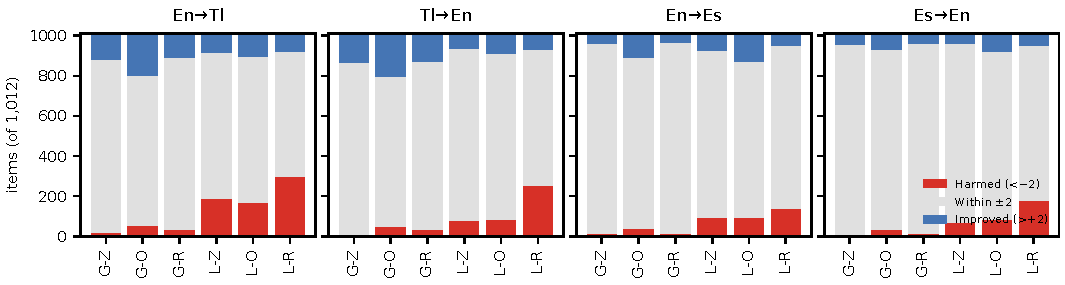
\includegraphics[width=\columnwidth]{figures/fig_bands.pdf}\caption{Improved ($>$+2 points), within-band, and harmed ($<-$2) devtest items per condition (G/L: GPT-4o Mini/Llama; Z/O/R: zero-shot/one-shot/reason-then-edit). Unchanged outputs lie within the band.}\label{fig:bands}\end{figure}}{}
\IfFileExists{generated/overediting_table.tex}{\begin{table}[t]
\centering\footnotesize
\caption{Protect-pool over-editing on devtest: over-edited items / protect-pool items per direction (protect: S0 COMET$\geq$0.90; over-edit: text changed and native COMET loss $>$0.02).}
\label{tab:overedit}
\setlength{\tabcolsep}{3pt}
\begin{tabular}{llrrrr}
\toprule
Editor & Strategy & En$\to$Tl & Tl$\to$En & En$\to$Es & Es$\to$En \\
\midrule
GPT-4o Mini & Zero & 3/234 & 3/377 & 3/275 & 1/293 \\
 & One & 6/234 & 26/377 & 7/275 & 12/293 \\
 & Reason & 5/234 & 13/377 & 3/275 & 4/293 \\
\midrule
Llama 3 8B & Zero & 42/234 & 35/377 & 29/275 & 26/293 \\
 & One & 35/234 & 37/377 & 28/275 & 33/293 \\
 & Reason & 57/234 & 107/377 & 32/275 & 51/293 \\
\bottomrule
\end{tabular}
\end{table}
}{}
\textbf{RQ3: over-editing of strong drafts.} Edit rate alone does not predict harm (Fig.~\ref{fig:bands}, Table~\ref{tab:overedit}). GPT-4o Mini one-shot changes 3{,}249 of 4{,}048 drafts (80\%) yet over-edits only 51 of 1{,}179 strong drafts (4.3\%); its zero-shot and reason-then-edit rates are 0.8\% and 2.1\%. Llama edits at similar rates but over-edits 11.2\% (zero-shot), 11.3\% (one-shot), and 20.9\% (reason-then-edit), up to 107 of 377 strong Tl$\to$En drafts. Llama harms more segments than it improves in 9 of 12 conditions; GPT-4o Mini improves more than it harms in all 12.

\textbf{RQ4: direction.} Direction effects are small and inconsistent: GPT-4o Mini gains more into English than out of English for every strategy in the Tagalog pair (e.g., $\DGptfourMiniZeroShotTagEng$ vs.\ $\DGptfourMiniZeroShotEngTag$ zero-shot), but not in the Spanish pair (one-shot $\DGptfourMiniKnnOneshotSpaEng$ into English vs.\ $\DGptfourMiniKnnOneshotEngSpa$ out of English).

\textbf{Robustness (exploratory).} No F1 decision changes under Bonferroni or Benjamini--Hochberg correction, or under Holm over both families jointly, and all 18 significant F1 effects have the same sign in COMET, BLEU, and chrF++. Wilson 95\% intervals keep the pooled over-editing rates apart (GPT-4o Mini at most 5.6\%, Llama at least 9.5\%), and among edited drafts every GPT-4o Mini condition harms at most 8.9\% of them, below the 9.9\% minimum for Llama.

\textbf{Summary.} GPT-4o Mini improved every condition and rarely damaged strong drafts; Llama improved none. The retrieved exemplar helped GPT-4o Mini most, and reason-then-edit ranked last for both editors in every direction.

\section{Discussion and Failure Analysis}
\textbf{Validity is part of the system.} Each condition is evaluated as deployed, including its fallback behaviour. Filtering to accepted responses would select a model-dependent subset and overstate editing benefits, so failure rates are reported alongside quality. The development pilot showed why: a strict diagnostic contract turned most Llama reason-then-edit outputs into the unchanged baseline, which is not restraint. \pending{held-out failure behaviour of the minimal contract, and what remains after controlling for it}.

\textbf{Average quality and fidelity can disagree.} During development, source-based inspection found an edit that changed a source-backed area figure while COMET rose, a schema-valid response that replaced a name with an unsupported one, and a source-consistent paraphrase that lost over 20 COMET points. These development cases motivate the preservation screens; they are illustrations, not population estimates. \pending{held-out preservation screen counts relative to the baseline (digits, capitalized tokens, language ID, length ratio, sentence counts) and two or three source-reviewed held-out cases}.

\section{Ethical Considerations and Reproducibility}
The study uses benchmark sentences and automatic evaluation without recruiting external raters. Its results do not establish suitability for medical, legal, or other consequential translation. Standard Spanish benchmark performance should not be generalized to local community or heritage varieties. LLM diagnostics can state unsupported errors with apparent confidence and should not be presented as expert explanations.

The public repository contains code, prompts, pinned configuration, reports, and numeric summaries. Raw benchmark text, full generations, vectors, model weights, credentials, and request identifiers are excluded from the public update. Access to underlying datasets and models remains subject to their respective terms. Norris artifacts remain separate from TRACE-MT; the earlier ICAI work is cited as prior methodology rather than merged into the experiment.

Draft prose and development analysis were prepared with AI assistance and checked against the supplied evidence. The project authors remain responsible for factual accuracy, attribution, and the venue's final disclosure requirements. Authorship, acknowledgments, funding wording, and publication metadata require PI confirmation before submission.

\section{Limitations and Ethical Considerations}
Two language pairs cannot identify a causal effect of resource level: language, direction, domain, and baseline quality are confounded. FLORES+ sources are largely English-original, so reverse directions involve translated source text. References are independent translations rather than minimal post-edits, so neither editing effort nor productivity is measured, and no bilingual human evaluation was conducted; COMET and the preservation screens are imperfect proxies. One open-weight checkpoint and one dated commercial snapshot do not represent all LLMs, pretraining exposure to the public benchmark cannot be ruled out, and deterministic settings do not guarantee identical remote behaviour. Fragment-level translation can lose cross-sentence context, and the reconstructed S0 fragment generation reproduced 412/421 multi-sentence development translations rather than all of them; every editor post-edits the same frozen devtest drafts, so the comparisons are unaffected.

The study uses public benchmark text and automatic evaluation only. Results do not establish suitability for medical, legal, or other consequential translation, and standard-Spanish results should not be generalized to community or heritage varieties. LLM diagnoses can state unsupported errors confidently and are not expert explanations. Code, prompts, frozen configuration, and numeric results are available (link withheld for anonymous review); benchmark text and generations are not redistributed. All GPT-4o Mini runs (development and held-out) cost about US\$1.26 at list token rates; Llama ran on one A100.~\pending{AI-use disclosure, only if the ICNLP submission instructions require it}

\section{Conclusions and Future Work}
On held-out FLORES+ data, LLM post-editing of a strong, sentence-split NLLB-200 baseline helped or harmed depending above all on the editor. GPT-4o Mini improved every direction, most with one retrieved exemplar; Llama 3 8B never improved and over-edited strong drafts, especially with reason-then-edit. Gains came from weak and mid-quality drafts rather than strong ones, the pair difference was only partly explained by baseline quality, direction effects were small, and explicit diagnosis improved neither editor. The study contributes a frozen, fully accounted four-direction evaluation and shows that average gains, preservation of strong drafts, and output validity are separate properties; all three should be reported before an LLM post-editor is deployed. Future work should test reference-free quality-estimation gates selected on development data, more language pairs and editors, document-level context, and bilingual human assessment.

\bibliographystyle{IEEEtran}
\bibliography{references}
\appendices
\section{Pinned Artifacts and Development Tables}
The public companion is \url{https://github.com/SHAZAN01/csudh-norris-ape-2026}. The measured prompts are candidate v2, with their complete identifier, exact bytes, schemas, sample IDs, revisions, and hashes in the reviewed candidate JSON under \path{config/phase3/}. The current freeze flag is false. Historical ``GPT pending'' fields inside the pre-GPT preparation provenance are retained as historical bytes, not as the current execution status.

Revision prefixes are listed below for readability; the manifest retains the complete immutable identifiers.
\begin{center}\small
\begin{tabular}{ll}\toprule
Artifact & Revision prefix \\\midrule
FLORES+ & \texttt{5fec6c13f9e5} \\
NLLB-200 3.3B & \texttt{1a07f7d19589} \\
LaBSE & \texttt{836121a0533e} \\
Llama model/tokenizer & \texttt{8afb486c1db2} \\
COMET & \texttt{2760a223ac95} \\\bottomrule
\end{tabular}
\end{center}

Retrieval used sentence-transformers 3.4.1 and FAISS CPU 1.9.0; it does not require a GPU FAISS build. Llama generation used vLLM 0.11.2, torch 2.9.0, and Transformers 4.57.1. Evaluation used torch 2.6.0+cu124, Transformers 4.49.0, unbabel-comet 2.2.7, NumPy 1.26.4, and SacreBLEU 2.6.0. Generation and evaluation are isolated environments; they should not be represented as a single tested installation.

The report's analysis signature begins \texttt{9d6830a0b9c7cc97}; the complete hash is recorded in the status manifest. Numeric audit artifacts contain all 24 conditions; the private original evidence contains raw completions and exact source/hypothesis/reference alignment. An audit script can reproduce lexical scoring from that evidence and check COMET aggregation without GPU inference.

\end{document}
